\documentclass[tikz,border=10pt]{standalone}
\usepackage{tikz}
\usetikzlibrary{angles,quotes,calc, intersections}

\begin{document}
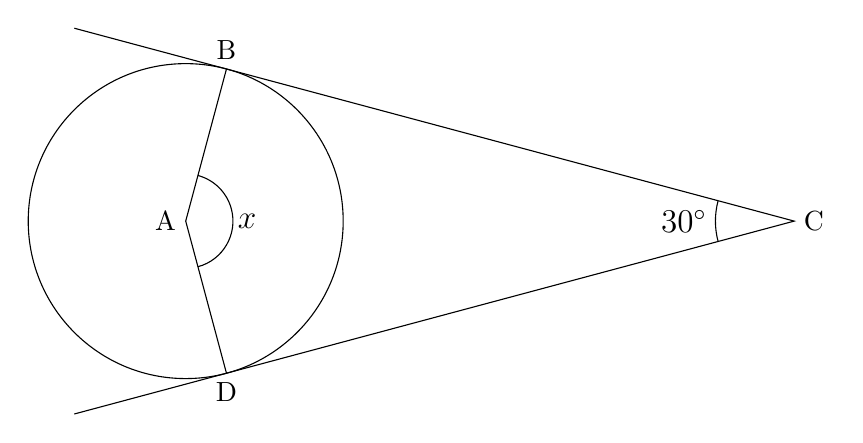
\begin{tikzpicture}

    % Define the center of the circle
    \coordinate (O) at (0,0);
    
    % Draw the circle
    \draw (O) circle (2cm);

    % Place points B and D on the circumference
    % The angle for B is -75 degrees (150/2) and for D is 75 degrees
    \coordinate (D) at ($(O) + (-75:2cm)$);
    \coordinate (B) at ($(O) + (75:2cm)$);

    % Draw points A,B, and D
    \node at (O) [anchor = east] {A};
    \node at (B) [anchor = south] {B};
    \node at (D) [anchor = north] {D};

    % Draw tangents from points B and D
    % Calculate tangent points
    \coordinate (T1) at ($(D)!4!-90:(O)$);
    \coordinate (T2) at ($(B)!4!90:(O)$);

    %extend tangents
    \coordinate (E1) at ($(D)!1!90:(O)$);
    \draw (D) -- (E1);
    \coordinate (E2) at ($(B)!1!-90:(O)$);
    \draw (B) -- (E2);
    % Find intersection point C
    \path [name path=line1] (B) -- (T2);
    \path [name path=line2] (D) -- (T1);
    \path [name intersections={of=line1 and line2,by={C}}];

    % Draw tangent lines
    \draw (B) -- (C) -- (D);

    % Label point C
    \node at (C) [right] {C};

    % Draw and label the angle at the center
    \draw (O) -- (B);
    \draw (O) -- (D);
    
    \pic [draw, "\large $30^\circ$", angle eccentricity=1.4, angle radius = 1cm] {angle = B--C--D};
    \pic [draw, "\large $x$", angle eccentricity=1.3, angle radius = 0.6cm] {angle = D--O--B};

\end{tikzpicture}
\end{document}
